\chapter{Design}

\subsection{General Description of the Architecture}

The architecture of the system follows a modular, component-based design to promote scalability, maintainability, and clear separation of responsibilities. It is organized into three main subsystems:

\begin{itemize}
    \item \textbf{Data Sources}: External components responsible for providing real-time data, event information, and public transport schedules.
    \item \textbf{Processing Core (Warehouse)}: Internal system modules that aggregate, analyze, and store incoming data, and coordinate responses.
    \item \textbf{Service and Interaction Layer}: Interfaces responsible for communicating results and actions to physical infrastructure and end users.
\end{itemize}

\vspace{1em}
The diagram below represents the structure and interactions between the system components:

\begin{center}
    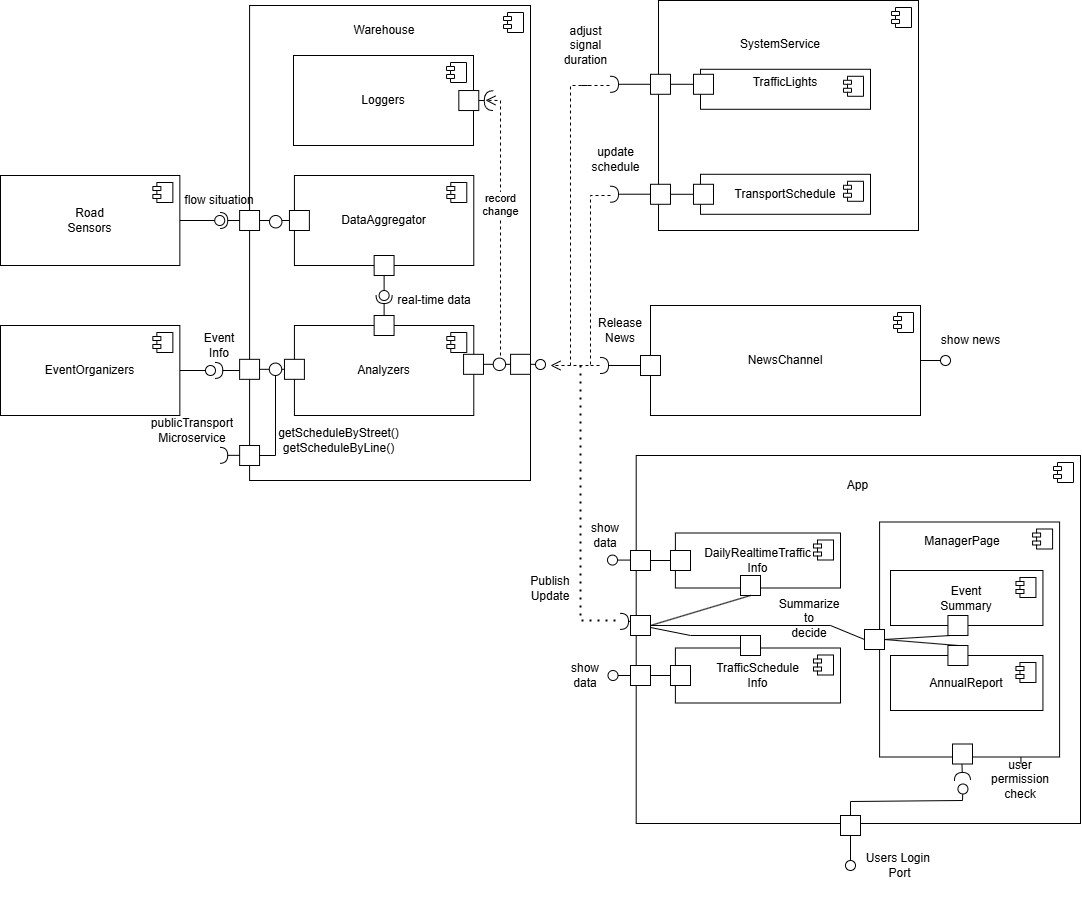
\includegraphics[width=0.95\textwidth]{Images/ComponentDiagram.png}
\end{center}

\paragraph{Component Descriptions:}

\begin{itemize}
    \item \textbf{Road Sensors}: Continuously stream real-time traffic flow data (e.g., congestion levels, vehicle counts) into the system.
    
    \item \textbf{Event Organizers}: Register events that may impact traffic. These inputs are handled by the system through the event dashboard.
    
    \item \textbf{Public Transport Microservice}: An external system providing transport timetables via API calls like \texttt{getScheduleByStreet()} and \texttt{getScheduleByLine()}.
    
    \item \textbf{Data Aggregator}: Collects raw traffic and event data from various sources and prepares it for analysis. Serves as a unified input hub.
    
    \item \textbf{Analyzers}: Responsible for processing different types of data, each dedicated to a specific functionality:

\begin{itemize}
    \item \textbf{Traffic Analyzer}: Handles real-time traffic data to detect congestion and trigger immediate adjustments to traffic lights (Type 1).
    \item \textbf{Pattern Analyzer}: Processes historical traffic data to identify long-term trends and suggest optimizations, such as route or schedule changes (Type 2).
    \item \textbf{Event Analyzer}: Assesses the potential impact of upcoming public events on traffic and transport systems, generating temporary plans and event news.(Type 3).
\end{itemize}

    
    \item \textbf{Loggers}: Record system actions, decisions, and configuration changes for auditing, traceability, and report generation.
    
    \item \textbf{SystemService}: Composed of two internal components:
    \begin{itemize}
        \item \textbf{TrafficLights}: Responsible for adapting signal timings based on analyzer output.
        \item \textbf{TransportSchedule}: Updates public transport schedules in response to congestion or planned events.
    \end{itemize}

    \item \textbf{News Channel}: Receives and displays information about upcoming events.

    \item \textbf{App}: The main interface for users, split into:
    \begin{itemize}
        \item \textbf{DailyRealtimeTrafficInfo}: Displays live traffic data to citizens.
        \item \textbf{TrafficScheduleInfo}: Shows updated public transport schedules.
        \item \textbf{ManagerPage}: Restricted area for traffic managers, with:
        \begin{itemize}
            \item \textbf{Event Summary}: Overview of past and upcoming events.
            \item \textbf{Annual Report}: Summary of yearly system activity and decisions.
        \end{itemize}
    \end{itemize}

    \item \textbf{Users Login Port}: Handles authentication and role-based access control, ensuring the right interface and permissions are applied.
\end{itemize}

Communication between modules is asynchronous and event-driven. This design allows the system to process multiple workflows in parallel (e.g., analyzing traffic while handling events) and maintain high performance under varying load conditions. Each module interacts via well-defined APIs or message-passing interfaces to support scalability and future extensions.

\newpage
\subsection{Sequence Diagrams}

This section presents three key sequence diagrams that illustrate the dynamic interactions between system components, services, and actors. Each sequence diagram corresponds to one of the three functional categories of the system: real-time congestion handling, pattern-based optimization, and event-based traffic planning.

The diagrams highlight:
\begin{itemize}
    \item The main flow of communication between modules.
    \item The triggering actions (e.g., sensor input, event registration).
    \item The system's behavior in processing, logging, and updating external interfaces.
\end{itemize}

\vspace{1em}
\subsubsection*{Type 1 – Adjust Traffic Flow (Real-Time Reaction)}

This diagram describes how the system processes real-time traffic data sent from sensors. The data is aggregated and analyzed, triggering adjustments to traffic light durations. All changes are recorded and traffic summaries are published in the app interface for citizens and managers.

\begin{center}
    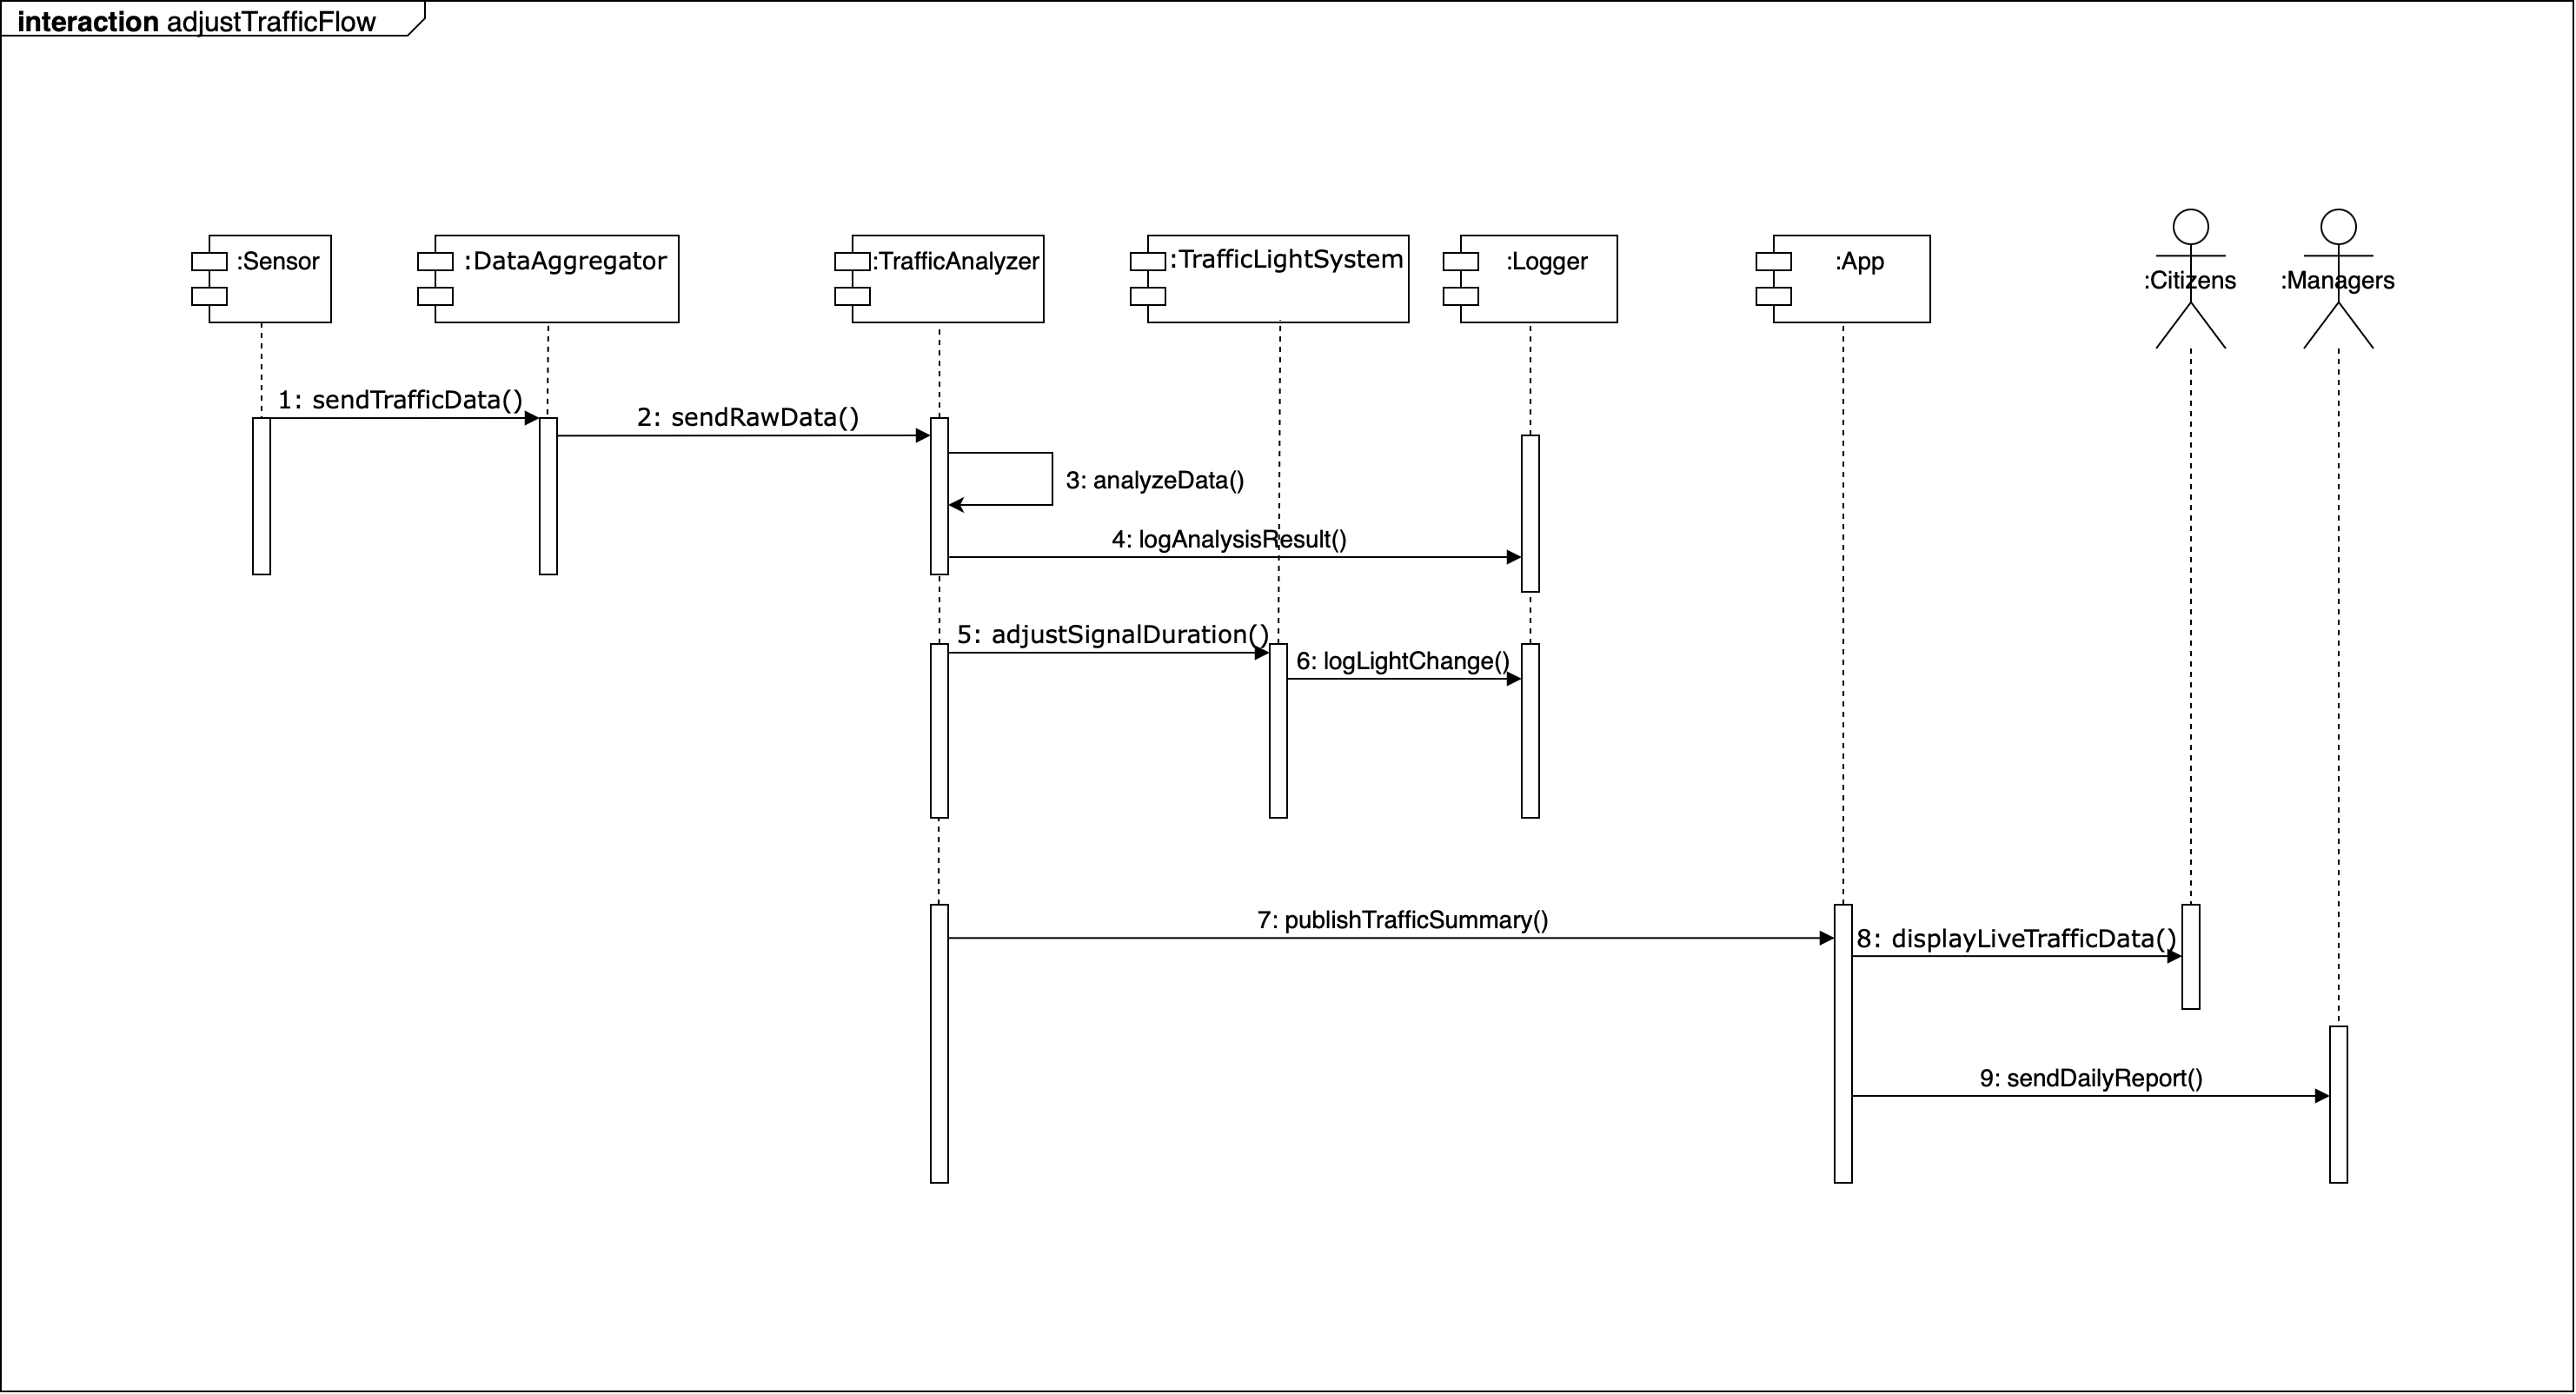
\includegraphics[width=1\textwidth]{Images/t1.sequence.png}
\end{center}





\newpage
\vspace{1em}
\subsubsection*{Type 2 – Suggest Pattern Optimization}

This interaction shows how historical traffic and schedule data are processed by the Pattern Analyzer to generate long-term optimization suggestions. Once approved by traffic managers, updates are made to public transport schedules and traffic light settings. The results are logged and made visible in the annual report.

\begin{center}
    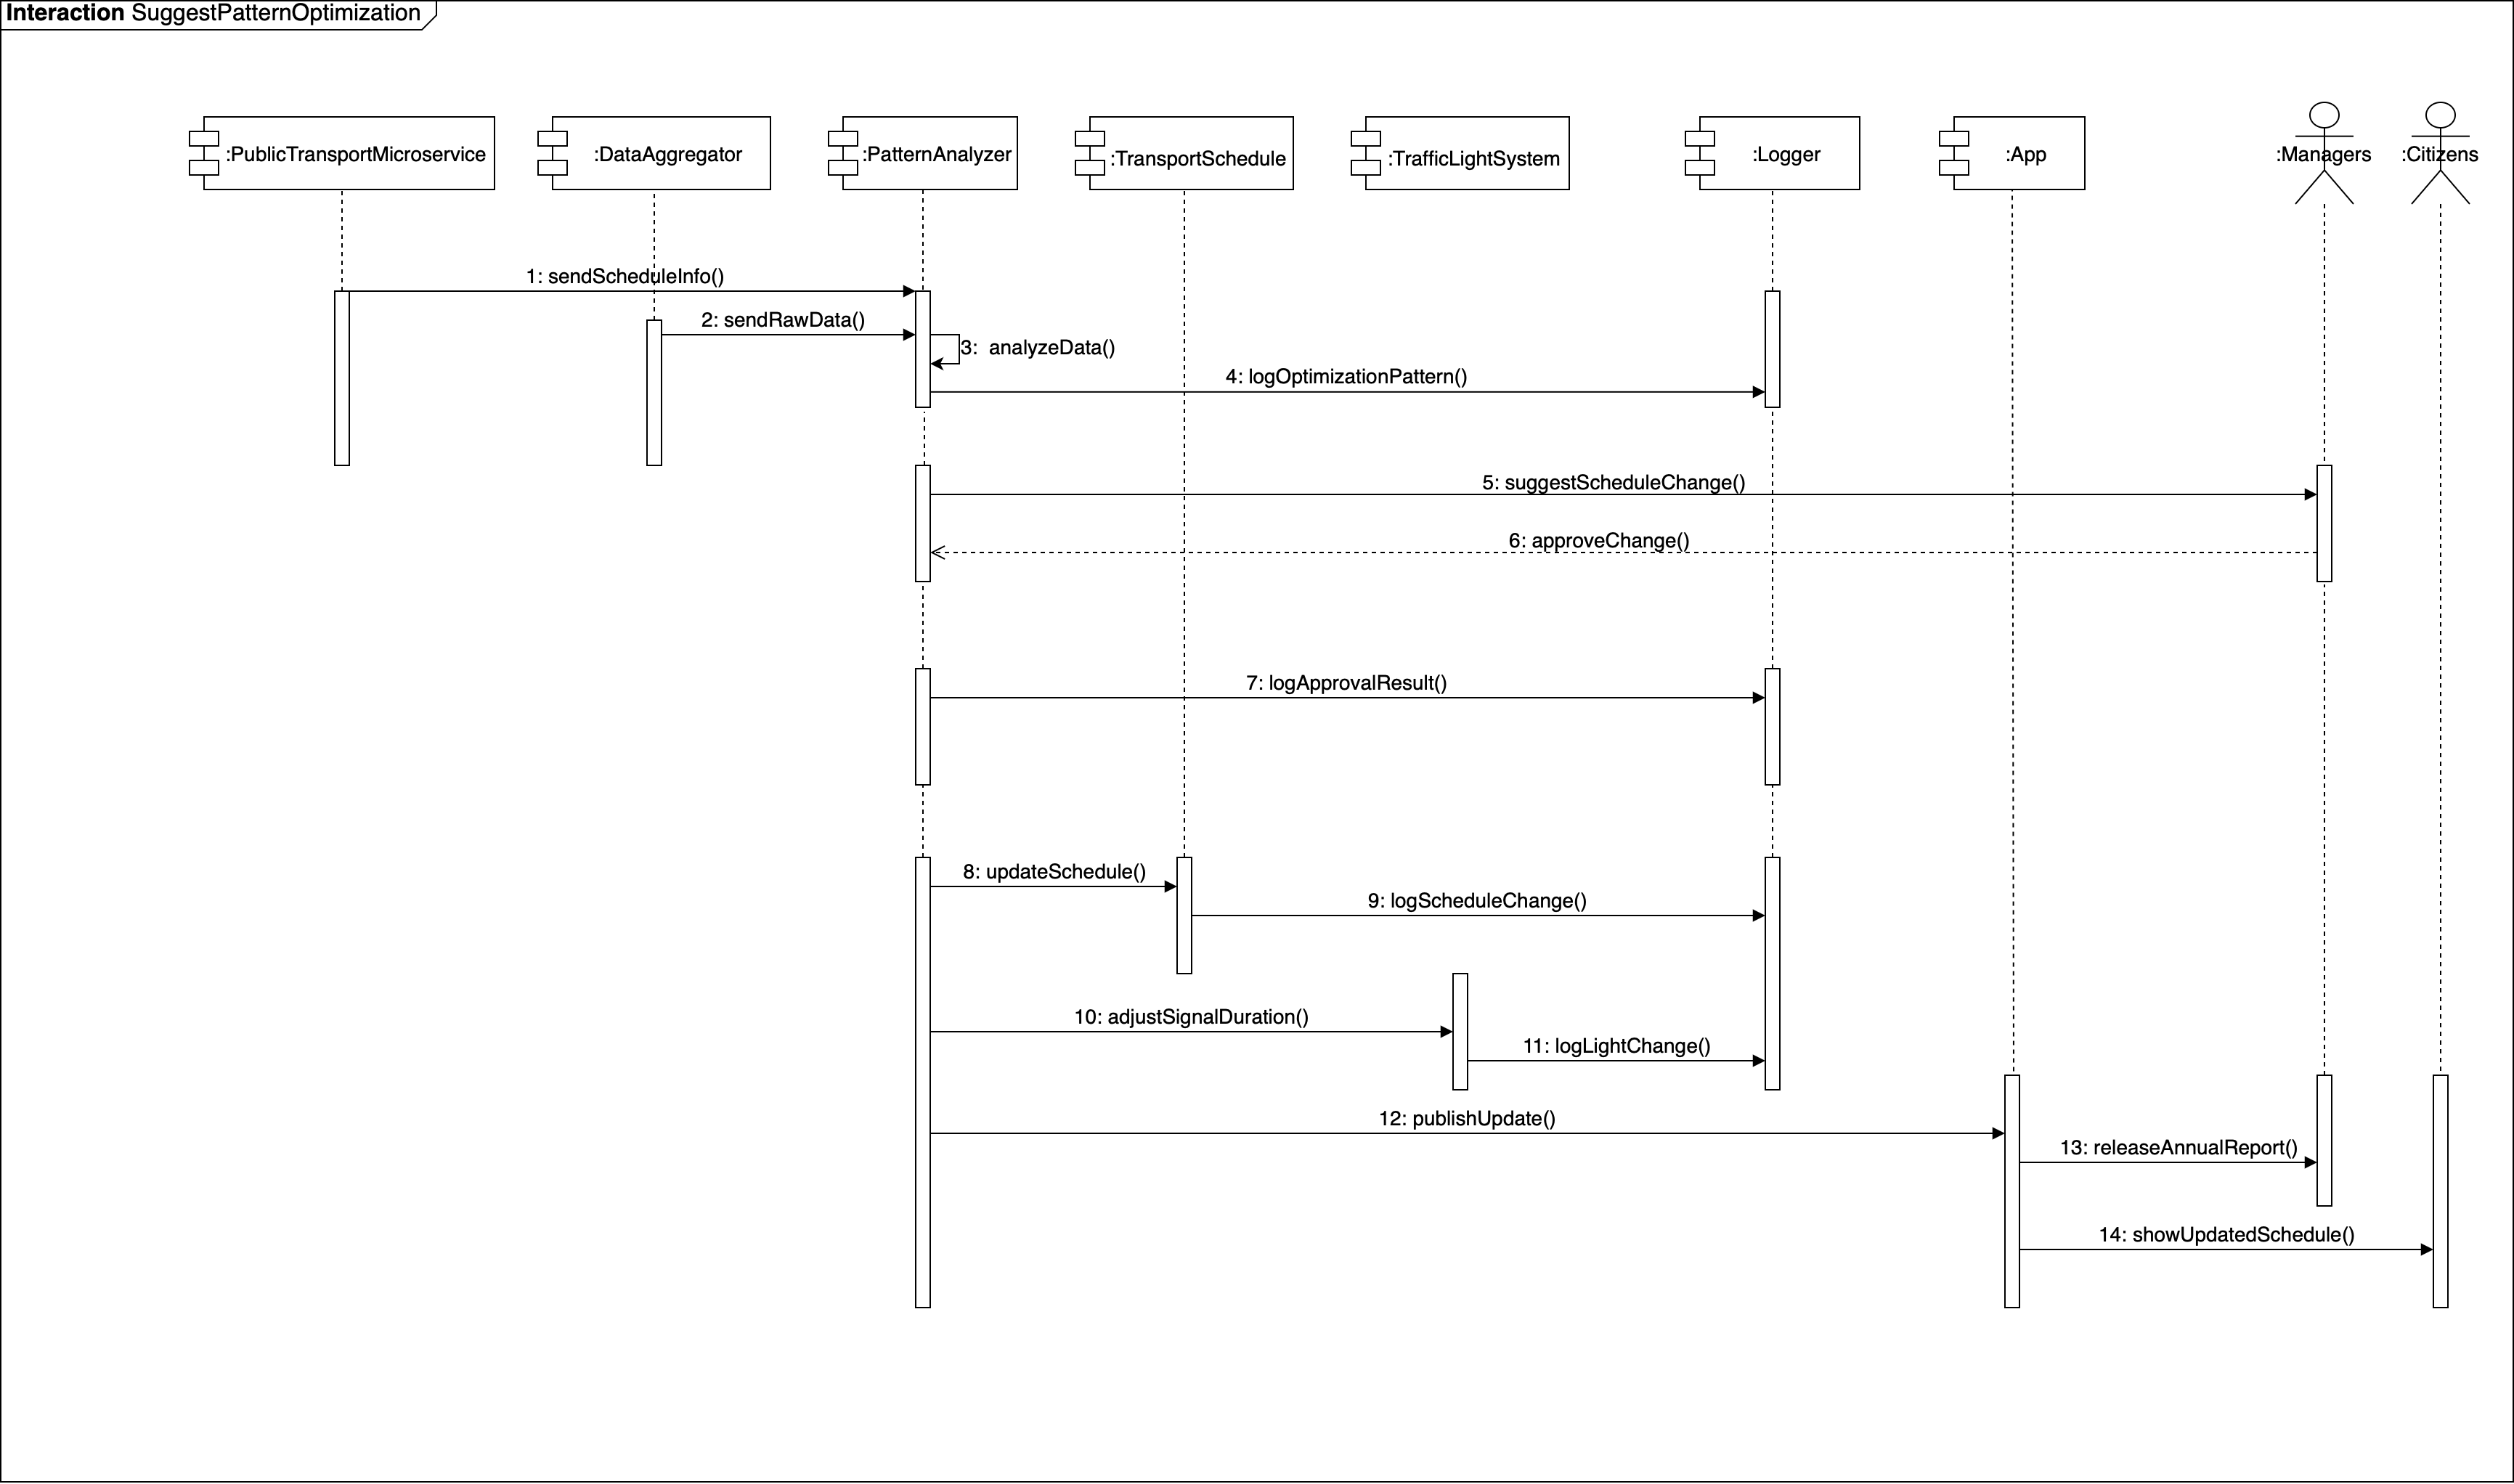
\includegraphics[width=1\textwidth]{Images/t2.sequence.png}
\end{center}

\newpage
\vspace{1em}
\subsubsection*{Type 3 – Change Transport for Event (Event-Based Adaptation)}

This diagram outlines how the system reacts when a new event is registered by an organizer. The Event Analyzer uses current and historical data to suggest temporary traffic and transport changes. Upon approval, configurations are updated, and notifications are sent to citizens through the app and news channels.

\begin{center}
    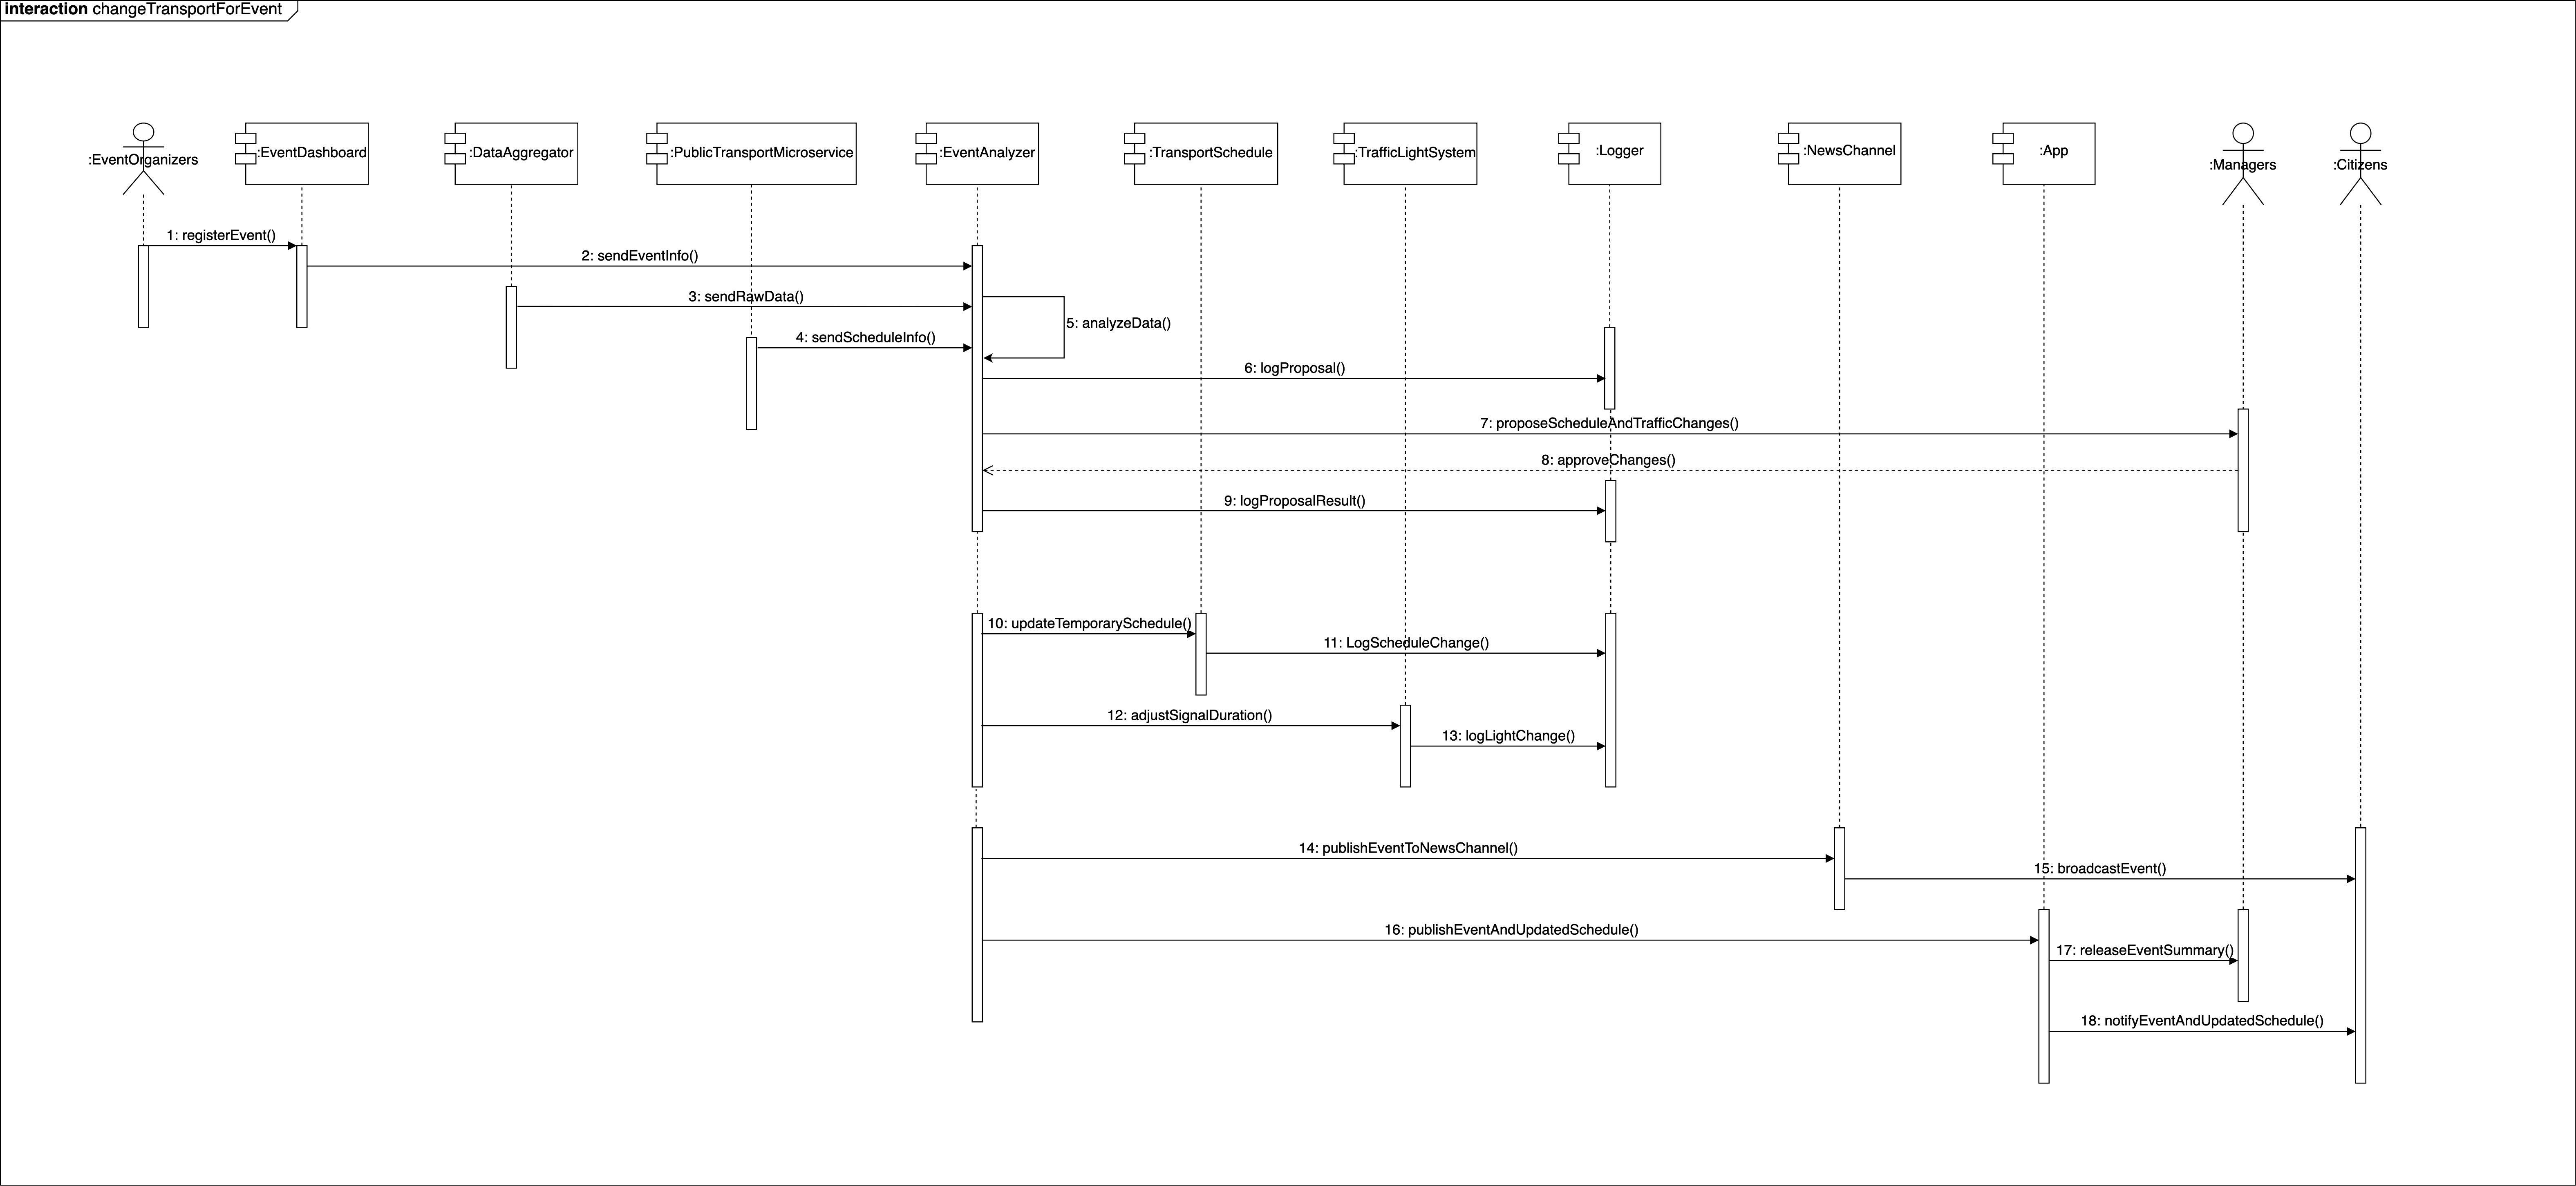
\includegraphics[width=1\textwidth]{Images/t3.sequence.png}
\end{center}




\newpage
\subsection{Critical Points and Design Decisions}

The following architectural and design decisions are directly based on the interactions illustrated in the sequence diagrams. They aim to ensure modularity, reliability, traceability, and scalability of the system:

\begin{itemize}
    \item \textbf{Dedicated Analyzers per Task}: Each main functionality (real-time updates, pattern analysis, and event planning) is handled by a specific analyzer. This separation supports maintainability and allows specialized processing logic for each type of analysis.

    \item \textbf{Centralized Data Aggregation}: All incoming data from external sensors are collected by a shared \texttt{DataAggregator}. This avoids redundancy and ensures consistency in the data used by different system modules.

    \item \textbf{Event-Driven Communication}: The system reacts to incoming data asynchronously. For example, signal adjustments or schedule updates are triggered automatically after analysis, without requiring manual input. This design improves responsiveness and system autonomy.

    \item \textbf{Approval Workflow for Critical Changes}: In Type 2 and Type 3 flows, the system generates suggestions rather than enforcing changes directly. Traffic managers must approve each proposal, ensuring control over modifications to public infrastructure.

    \item \textbf{Separation of Analysis and Execution}: The process of analyzing data and generating suggestions is clearly separated from the components responsible for applying changes. This design reduces the risk of unintended behavior and improves traceability.

    \item \textbf{Comprehensive Logging}: All major actions such as approvals, changes to signal durations, and schedule updates are recorded by the \texttt{Logger}.

    \item \textbf{Role-Specific Interfaces}: The system interface (App) provides different functionalities depending on the user role. Citizens receive real-time updates and routing suggestions, as well as the incoming events, while managers access dashboards to review and check reports.

    \item \textbf{Scalability and Parallel Processing}: The architecture supports multiple independent data flows, as shown in the sequence diagrams. This enables the system to handle concurrent traffic conditions and events without performance degradation.
\end{itemize}
